% thesis.tex
%
% This file is root file for an example thesis written using the
% IIT Guwahati LaTeX Style file.

% The IIT Guwahati LaTex Style is a modified
% version of IIT Bombay LaTex Style created by
% Dr. Amey Karkare (21 June 2007).
%
% Required permissions have been taken from Dr. Karkare in order to
% create the IIT Guwahati LaTex Style using his original work.
% Revision done by: Mandar Kulkarni, EEE Department, IIT Guwahati
% Further revised by Dr. Sonali Chouhan, EEE Department, IIT Guwahati (16/04/2016)

%=====================================================================
% Read: README.txt for more information
%=====================================================================

%=====================================================================
% DOCUMENT STYLE
%=====================================================================
% IITG Thesis format default settings are:
%   12pt, one-sided printing on a4 size paper
\documentclass{iitgthesis}
% For two-sided printing, with Chapter starting on odd-numbered pages,
% use the following line instead:
%%\documentclass[openright,twoside]{iitgthesis}

%=====================================================================
% OPTIONAL PACKAGES
%=====================================================================
% To include optional packages, use the \usepackage command.
% For e.g., The package epsfig is used to bring in the Encapsulated
%    PostScript figures into the document.
%    The package times is used to change the fonts to Times Roman;
%=====================================================================
\usepackage{epsfig}
\usepackage{stackrel}
\usepackage{epsf}
\usepackage{amssymb}
\usepackage{amsthm}
\usepackage{graphicx}
\usepackage[english]{babel}
\usepackage{mathrsfs}
%\usepackage{fancyhdr}
\usepackage{verbatim}
\usepackage{amsmath,amssymb}

\usepackage{cite}
\usepackage{multirow,tabularx}
\usepackage{ifthen}
% Add these after the document class declaration
\usepackage{times}
\DeclareMathAlphabet{\mathpzc}{OT1}{pzc}{m}{it}


\usepackage{amssymb}
%\usepackage{dsfont}
%\usepackage{stmaryrd}
\usepackage{amsmath}
\usepackage{mathrsfs}
%=====================================================================
%  Single counter for theorems and theorem-like environments:
%=====================================================================
\newtheorem{thm}{Theorem}[section]
\newtheorem{theorem}{{\bf Theorem}}
\newtheorem{lemma}{{Lemma}}
\newtheorem{proposition}[theorem]{Proposition}
\newtheorem{corollary}{{\bf Corollary}}
\newtheorem{result}{{\bf Result}}

%=====================================================================
% NEW COMMANDS DEFINED FOR A EASY TO READ CODE
% You are free to add your own set of new commands here
%
\newcommand{\brac}[1]{\left({#1}\right)}
\newcommand{\sbrac}[1]{\left[{#1}\right]}
\newcommand{\cbrac}[1]{\left\{{#1}\right\}}
\newcommand{\expc}[2][]{E_{#1}\left[{#2}\right]}

% End of Preamble, start of document
%
\begin{document}

%=====================================================================
% Include the prelude for Title page, abstract, table of contents, etc
% You need to modify it to contain your details
% prelude.tex
%   - titlepage
%   - dedication (optional)
%   - approval sheet
%   - course certificate
%   - table of contents, list of tables and list of figures
%   - nomenclature
%   - abstract
%============================================================================


\clearpage\pagenumbering{roman}  % This makes the page numbers Roman (i, ii, etc)



% TITLE PAGE
%   - define \title{} \author{} \date{}
\title{VLSI Architectures for Long Short Term Memory Networks}
\author{Author}
\date{November 2018}

%  - Roll number, required for title page, approval sheet, and
%    certificate of course work
\rollnum{150102077) \vspace{0.5}   (Roll No. 150102060}
\author{Krishna Praveen Yalamarthy \hspace{1}   Saurabh Dhall}

%   - The default degree is ``Doctor of Philosophy''
%     (unless the document style msthesis is specified
%      and then the default degree is ``Master of Science'')
%     Degree can be changed using the command \iitbdegree{}
\iitgdegree{Bachelor of Technology}

%   - The default report type is preliminary report.
%      * for a PhD thesis, specify \thesis
\thesis
%      * for a M.Tech./M.Phil./M.Des./M.S. dissertation, specify \dissertation
%\dissertation
%      * for a DIIT/B.Tech./M.Sc.project report, specify \project
%\project
%      * for any other type, use  \reporttype{}
%\reporttype{ReportType}

%   - The default department is ``Unknown Department''
%     The department can be changed using the command \department{}
\department{DEPARTMENT OF ELECTRONICS \& ELECTRICAL ENGINEERING}

%    - Set the guide's name
\setguide{Prof. Rafi Ahmed}

%   - once the above are defined, use \maketitle to generate the titlepage
\maketitle

%--------------------------------------------------------------------%
% APPROVAL SHEET
%   - for final thesis, you need Approval Sheet. So, uncomment the
%     \makeapproval command.
%     it should come after dedication, if dedication is
%     present. Otherwise it is the first page after title page.
%\makeapproval


%--------------------------------------------------------------------%
% COPYRIGHT PAGE
%   - To include a copyright page use \copyrightpage
% \copyrightpage

%--------------------------------------------------------------------%

% ACKNOWLEDGMENTS (optional)
\begin{acknowledgments}
Sample Acknowledgement
\end{acknowledgments}


% ABSTRACT
\begin{abstract}

Long Short Term Memory Networks, which are a modification of the traditional Recurrent Neural Networks, have gained widespread integration into commercial applications to accomplish tasks in the domains of speech recognition, handwriting recognition and are currently deployed in many embedded devices. These networks are computationally expensive and require considerable memory and storage bandwidth which restricts their further use in resource constrained devices. There has been considerable work on optimizing these networks at an algorithmic level, yet there is little to no work being done to reduce the computational complexity on an architectural level using VLSI-DSP techniques. Intially, state-of-art model compression techniques such as Pruning, Quantization, Knowledge distillation are exlpored to decrease the size of the model itself. The next major component of the thesis concentrates on using Distributed Arithmetic to trade computational complexity with ROM lookups. 

\end{abstract}


%--------------------------------------------------------------------%
% CONTENTS, TABLES, FIGURES
\tableofcontents
%\listoftables
\listoffigures

%--------------------------------------------------------------------%
% NOMENCLATURE
%\begin{nomenclature}
%\begin{description}
%\item{\makebox[0.75in][l]{{SN1}}} Sample Nomenclature 1

%\item{\makebox[0.75in][l]{{SN2}}} Sample Nomenclature 2

%\end{description}
%\end{nomenclature}

\cleardoublepage\pagenumbering{arabic} % Make the page numbers Arabic (1, 2, etc)


%=====================================================================
% Include the technical part of the report
\chapter{Introduction}
\label{chap:intro}
\section{VLSI Design Flow}
The development cycle of any digital IC is governed by a few fundmanetal steps or processes that are sequentially followed. The first step begins with designing an algorithm to solve the problem and meet the requirements. Coming up with an algorithm is followed by designing an architecture which can be realized on hardware that is feasible in the desired resource-constrained use case. Different architectures can be proposed for the same algorithm which can be further optimized at the gate level. As shown in the figure \ref{fig:vlsi}, in order to fully exploit the benefit of having an ASIC design, after the gate level modelling, transistor level optimizations are also important. The last stage of the design cycle ends with modifications at the device level.

A small modification at an earlier level in the design flow can lead to a significant change at a later level. A single multiplier that could be eliminated at the architectural level would lead to saving thousands of transistors indicating the significance of higher level optimizations. Since the effects of an optimization are reflected in the following stages, it is essential to fully explore the various possible models or designs.

\begin{figure}[h]
\label{fig:vlsi}
	\caption{VLSI Design Flow}    
    \centering
    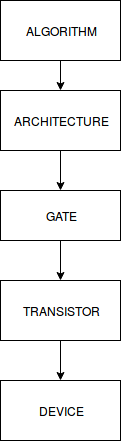
\includegraphics[width=0.1\textwidth]{vlsi_dESIGN}
\end{figure}

\section{Machine Learning}
The field of machine learning is not one that is new. These algorithms have been in existence for a long time although only in recent years they have come into popularity, especially neural networks and deep learning, thanks to the rapid increase in computational power. The GPU has aided in increasing the scale of these models to actually work effectively on real-world tasks. While major strides have been made in improving these algorithms by extensive training and refinement at an algorithmic level, research into architectural changes has been limited. \\
Due to recent advancements in compute power in embedded/mobile device, there is now a possibility of implementing these computationally expensive models on devices with a tighter power, memory and compute constraint than was previously there on non-mobile devices. \\
Indicative of the growing interest in embedded implementations of such networks, in the last couple of years there have been some works on FPGA deployment of LSTMs but none of them seem to leveraging the VLSI digital signal processing techniques for optimization.% [refs to these works] 
VLSI DSP techniques such as systolic arrays, unfolding, distributed arithmetic, CORDIC, pipelining etc., have been in use for the past 30 years for the fields of communication, filters, image processing lend themselves really well for machine learning algorithms as well. Recent work inspired by these techniques optimize Support Vector Machines and Convolutional Neural Networks.%[refs to Rafis papers] 
One branch of neural networks that is explicitly suited for tasks that are applicable in mobile devices are Recurrent Neural Networks. These networks are suited for data that is sequential in nature and have been shown to be effective at tasks such as handwriting recognition and generation, speech and speaker recognition, language modelling, speech synthesis to name a few. \\

\section{Literature Review}
A specialised version of the RNN that is extremely popular for commercial application is the Long Short Term Memory network (LSTM). It is adept at establishing long term dependencies in data . As of 2016, many software giants such as Google, Apple and Microsoft had LSTMs as a fundamental unit in their products. Google incorporated LSTMs for the speech recognition task on the handheld device and also into their smart assistant as well as Google Translate. \\
\\
The typical computational power required by LSTMs is demanding. The challenge of deploying these models is further increased due to the size of the models themselves which needs to be stored locally to fully execute these tasks. 

-original paper
-lstm odyssey
-compression papers
-no proper application of VLSI DSP in this field. can lead to significant improvement to help deploy on devices.

\section{Problem Formulation}
Our goal is to leverage both the best of the available algorithmic optimizations or a combination of those followed by VLSI DSP techniques that are suited to exploit some unique properties of LSTM.
% change to third person
We will first go through the preliminaries that establish the algorithm of Long Short Term Memory Networks. We will then systematically go through the different levels of optimization, from algorithmic to an architectural level, that can be applied to these networks.
        % Chapter 1: Introduction
%\include{literature}         % Chapter 2: Literature survey
%\include{system}             % Chapter 3: System model and formulating the problem statement
%\include{analysis}           % Chapter 4: Analysis
%\include{results}            % Chapter 5: Simulation and Results
%\include{conclusion}         % Chapter 6: Finally the summary & conclusions

%=====================================================================
% APPENDIX
%  Appendices, if any, must precede the cited literatures.
%  Appendices shall be numbered in Roman Capitals (e.g. Appendix IV)

%% \appendix
%% \include{appendix_something}

%=====================================================================
% BIBLIOGRAPHY
%   This should follow the appendices, if any, otherwise summary and
%   conclusions chapter.
% Choose your bibliography style
% plain is the basic style, others include ieeetr, siam, asm, etc
%\bibliographystyle{plain}
% Add the bib file
%% \bibliography{bibfile}
\begin{thebibliography}{9}
\begin{small}

\bibitem{ref:FCC}
``Spectrum Policy Task Force Report,'' {\em Federal Commun.\ Commission,\ Tech.\ Rep.}, Nov.~2002.\\
 Available at http://hraunfoss.fcc.gov/edocs\_publish/attachmatch/DOC-228542A1.pdf

\bibitem{ref:haykin}
S. Haykin, ``Cognitive Radio: Brain Empowered Wireless Communications,'' {\em IEEE Journal on Selected Areas in Communication}, Vol.~23, No.~2, pp.~201-�220, Feb.~2005.

\end{small}
\end{thebibliography}
%=====================================================================
% PUBLICATIONS
%  publications if any may be listed after the literature cited.
%% \include{mypubs}

%=====================================================================


\end{document} 
